\documentclass[12pt]{article}

\usepackage[utf8]{inputenc}
\usepackage[T1]{fontenc}
\usepackage{amssymb}
\usepackage{amsmath}
\usepackage{geometry}
\usepackage{parskip}
\usepackage{setspace}
\usepackage{graphicx}
\usepackage{hyperref}
\usepackage{indentfirst}
\usepackage{booktabs}
\usepackage{multirow}

\geometry{a4paper, margin=1in}
\onehalfspacing{}
\setlength{\parindent}{2em}
\setlength{\parskip}{0.5\baselineskip}

\title{A study on the Detection of Gender Antagonism Tendency in Chinese Social Media Based on CMLG Model}
\author{%
Author: \underline{Yonghao Yang} \\
Institution/School: \underline{Wuhan University} \\
Email: \underline{13235595638@163.com}%
}
\date{\today}

\begin{document}

\maketitle

\begin{abstract}
Gender-antagonistic discourse pervades Chinese social media, yet automatic detection remains unreliable due to the informal register, creative character-play, and noisy human annotations typical of this domain. We propose CMLG, a model that fuses CKBERT contextual embeddings, BGE dense embeddings, pinyin phonetic vectors, and wubi structural vectors through learnable feature-level attention, and classifies the fused sequence with a Bi-GRU backbone. To address label noise---which we identify as the dominant performance bottleneck---we introduce a cleaning pipeline in which three heterogeneous LLMs (Qwen2.5-72B, GLM-4-32B, DeepSeek-V3) independently vote on every sample. Ablation across five feature configurations and three dataset versions (original, majority-vote cleaned, unanimous-agreement cleaned) reveals two key findings: (1) label cleaning raises macro F1 from 0.7824 to 0.9007 (+12pp), consistently improving all tested models by 9--14pp; (2) Chinese-specific orthographic features (pinyin, wubi) are ineffective on noisy labels but become the strongest configuration once labels are cleaned, indicating that annotation quality gates the learnability of fine-grained linguistic cues.
\end{abstract}

\noindent\textbf{Keywords:} gender antagonism; deep learning; LLM-assisted data cleaning; feature-level attention fusion; Chinese NLP

\section{Introduction}
Gender-oriented hostility on social media has become a pressing societal concern across many countries [1,2]. In the Chinese-speaking internet, platforms such as Weibo, Douyin, and Zhihu host millions of daily comments, a fraction of which contain targeted attacks against specific gender groups. Research on the psychological consequences of exposure to such content has documented increased anxiety and polarization among younger cohorts [2], while sociological analyses link the phenomenon to declining willingness to marry or bear children [2,3]. Fontanella et al.\ [3] note that misogynistic discourse online can normalize hostility and spill over into offline behavior, making automated detection a prerequisite for effective content governance.

English-language sexism detection has matured considerably, with shared tasks, benchmark datasets, and a variety of transformer-based models [4--7,16,17]. Chinese online discourse, however, presents additional linguistic challenges. Users routinely employ homophonic substitution---replacing a sensitive word with a character that sounds identical but carries a different literal meaning---and shape-similar character swaps based on the visual similarity of Chinese glyphs [9]. These evasion tactics defeat keyword filters and weaken models that rely solely on semantic embeddings, because the surface form of the text deliberately diverges from its intended meaning.

A further complication is annotation quality. Subjective labeling tasks such as hate speech and sexism detection are known to produce noisy ground truth [19,20], and our preliminary analysis of the SWSR corpus [8] confirms that a non-trivial fraction of its labels are inconsistent with consensus judgments from large language models. This observation motivates the data-cleaning component of our approach.

We define ``gender antagonism tendency'' as the directional stance an expression conveys toward a gender group, rather than its hostility intensity alone [2]. Although a three-class formulation (pro-male/anti-female, pro-female/anti-male, neutral) was initially planned, the available SWSR corpus supplies only binary labels. Preliminary trials also showed that current LLMs can exhibit gender biases that make them unsuitable as sole annotators for fine-grained directional labeling. We therefore work with a binary task---gender-antagonistic (label~1) vs.\ neutral (label~0)---and leave directional classification for future work.

This study makes three contributions. First, we design CMLG (CKBERT-based Multi-feature LLM-enhanced Bi-GRU), which fuses contextual, dense-semantic, phonetic, and structural embeddings through learnable feature-level attention, combining pretrained language model representations with Chinese-specific orthographic cues that target the evasion tactics described above. Second, we build an LLM-assisted data cleaning pipeline based on three-model majority voting, producing two re-labeled dataset variants that enable controlled study of how label quality affects downstream classification. Third, through ablation experiments spanning three dataset versions, five feature configurations, and two baselines, we show that label quality---not model architecture or feature engineering---is the dominant performance factor, and that Chinese orthographic features shift from useless to most valuable once annotation noise is removed.

\section{Literature Review}

\subsection{Hate Speech and Gender Hostility Detection}
Automated hate speech detection has progressed rapidly in the past decade. Fortuna and Nunes [16] provide a comprehensive survey of text-based approaches, categorizing methods from keyword matching and bag-of-words classifiers through deep neural networks. A persistent challenge highlighted in their survey is the boundary between offensive language and genuinely hateful content. Davidson et al.\ [17] formalize this distinction and demonstrate that many classifiers conflate the two categories, achieving high recall on offensive posts but poor precision on hate speech. This ambiguity is equally problematic in gender-antagonism detection, where sarcastic, ironic, or exaggerated statements about gender may or may not constitute hostility depending on context.

Within the gender-specific strand, Gutam et al.\ [4] coupled BERT with community-enhanced annotations and reduced manual moderation workload by 40\%, illustrating the practical value of transformer-based classifiers for platform governance. Singh et al.\ [5] constructed the first Hindi--English code-mixed misogyny benchmark and found that multilingual BERT outperformed monolingual baselines, underscoring the importance of pretraining on the target language family. Vivekananda et al.\ [6] experimented with BERT--classical-ML hybrids augmented by weak supervision, reporting that ensemble strategies can partially compensate for scarce labeled data. Mohasseb et al.\ [7] combined LDA topic models with Sentence-Transformer embeddings for data augmentation, emphasizing cross-corpus transferability as a desirable but difficult goal. Luo et al.\ [1] provide the most recent survey of multimodal and multilingual sexism detection, identifying a gap in Chinese-language coverage and calling for dedicated Chinese datasets and models.

\subsection{Chinese-Language Sexism Detection}
Chinese-language research in this field remains at an early stage compared to its English counterpart. Jiang et al.\ [8] released the SWSR dataset, the first Chinese corpus annotated for online sexism at three granularities---binary presence, type of sexism, and target gender. Despite its value as a pioneering resource, SWSR was annotated by a small team, and the authors acknowledge inter-annotator disagreement on borderline cases; our cleaning experiments quantify this disagreement at roughly 18\% of the corpus. Ma et al.\ [9] extended SWSR by incorporating pictographic and structural character features (inspired by the Wubi input method), reporting a 5.19pp F1 gain over a text-only baseline. Their work was the first to demonstrate that Chinese-specific orthographic information carries discriminative signal for sexism detection, a finding we build upon with a more principled multi-stream fusion that separates phonetic from structural cues and weights them adaptively. Sun et al.\ [18] investigated fine-tuning strategies for BERT on several Chinese text classification benchmarks and showed that task-specific intermediate training and layer-wise learning rates can yield non-trivial gains; their recommendations inform our BERT baseline configuration.

\subsection{Label Noise in Text Classification}
Noisy labels are a pervasive problem in supervised text classification, especially when annotations are crowdsourced or performed by non-experts. Fr\'{e}nay and Verleysen [19] survey classical approaches to learning under label noise, grouping them into noise modeling, sample filtering, and robust loss design. Their analysis shows that even moderate noise rates (10--20\%) can substantially degrade classifier performance, particularly for minority classes. Song et al.\ [20] extend the survey to deep-learning-specific techniques, covering sample re-weighting, co-teaching, meta-learning, and mixup regularization. Both surveys note that no single strategy dominates across all settings, and that the optimal approach depends on noise rate, noise type (symmetric vs.\ asymmetric), and class balance.

Our pipeline takes the filtering route: rather than designing a noise-tolerant learner, we use multi-LLM consensus to identify and correct likely mislabeled samples before training. This approach is conceptually simple and has the advantage of producing a reusable cleaned dataset that benefits any downstream model, as our experiments confirm.

\section{Methodology}

\subsection{Dataset}

\subsubsection{Data Source and Problem Formulation}
We use the SWSR dataset [8], retaining the \texttt{comment\_text} and \texttt{label} columns. The corpus contains 8{,}969 samples: 5{,}876 gender-neutral (label~0, 65.5\%) and 3{,}093 gender-antagonistic (label~1, 34.5\%). The task is binary text classification.

\subsubsection{LLM-Assisted Label Cleaning}
\label{sec:llm-cleaning}
To quantify and reduce annotation noise, we designed a cleaning pipeline based on three-model majority voting. Three LLMs---Qwen2.5-72B-Instruct, GLM-4-32B-0414, and DeepSeek-V3---each independently classify every sample using a structured Chinese prompt (Appendix~A). Predictions are aggregated by majority rule, yielding two cleaned variants:

\begin{itemize}
    \item \textbf{Cleaned-Full} (8{,}962 samples): all samples with a valid majority vote, relabeled accordingly. The label distribution shifts to 5{,}419 neutral (60.5\%) and 3{,}543 opposing (39.5\%).
    \item \textbf{Cleaned-HighConf} (6{,}793 samples): only samples where all three models unanimously agree, providing the highest label confidence. The distribution is 4{,}219 neutral (62.1\%) and 2{,}574 opposing (37.9\%).
\end{itemize}

Comparing original and cleaned labels, roughly 18.3\% of the original annotations disagree with the LLM consensus---a non-trivial noise rate. Table~\ref{tab:llm-stats} reports the per-model statistics.

\begin{table}[htbp]
\centering
\caption{Per-LLM cleaning statistics on the full 8{,}969-sample corpus.}
\label{tab:llm-stats}
\begin{tabular}{lccc}
\toprule
 & Qwen2.5-72B & GLM-4-32B & DeepSeek-V3 \\
\midrule
Valid responses & 87.4\% & 99.5\% & 99.5\% \\
Agreement w/ original labels & 75.3\% & 80.2\% & 81.5\% \\
Agreement w/ majority vote & 87.4\% & 96.1\% & 90.6\% \\
\midrule
Pairwise agreement & \multicolumn{3}{c}{Qwen--GLM: 84.5\%, Qwen--DS: 77.0\%, GLM--DS: 86.7\%} \\
Unanimous agreement & \multicolumn{3}{c}{6{,}793 / 8{,}969 samples (75.7\%)} \\
\bottomrule
\end{tabular}
\end{table}

\subsection{Feature Extraction}
Four parallel streams capture complementary aspects of each input text. Table~\ref{tab:features} summarizes the streams.

\begin{table}[htbp]
\centering
\caption{Feature streams used in CMLG.}
\label{tab:features}
\begin{tabular}{lllp{5.8cm}}
\toprule
Stream & Encoder & Dim & Rationale \\
\midrule
CKBERT ($v_c$) & CK-BERT [10,12] & $T \times 1024$ & Knowledge-enhanced contextual embeddings; primary semantic channel. \\
BGE ($v_b$) & BGE-base-zh-v1.5 [13] & $T \times 768$ & Dense sentence-level semantics from a separate pretraining objective. \\
Pinyin ($v_p$) & Word2Vec [14] & $T \times 256$ & Captures homophonic substitution (e.g., swapping sensitive words for characters that sound alike). \\
Wubi ($v_w$) & Word2Vec [14] & $T \times 256$ & Captures shape-similar character substitution via Wubi keystroke sequences. \\
\bottomrule
\end{tabular}
\end{table}

For CKBERT and BGE, character-level embeddings are recovered through offset mapping; where a subword token spans multiple characters, embeddings are averaged. Pinyin and wubi Word2Vec models are trained on the corpus itself and L2-normalized per token. CKBERT and BGE embeddings are extracted once and cached; pinyin and wubi models are retrained per dataset variant to reflect corpus composition differences.

\subsection{Model Overview}
Figure~\ref{fig:architecture} illustrates the full CMLG pipeline, from multi-stream feature extraction through attention fusion to the final classifier.

\begin{figure}[htbp]
\centering
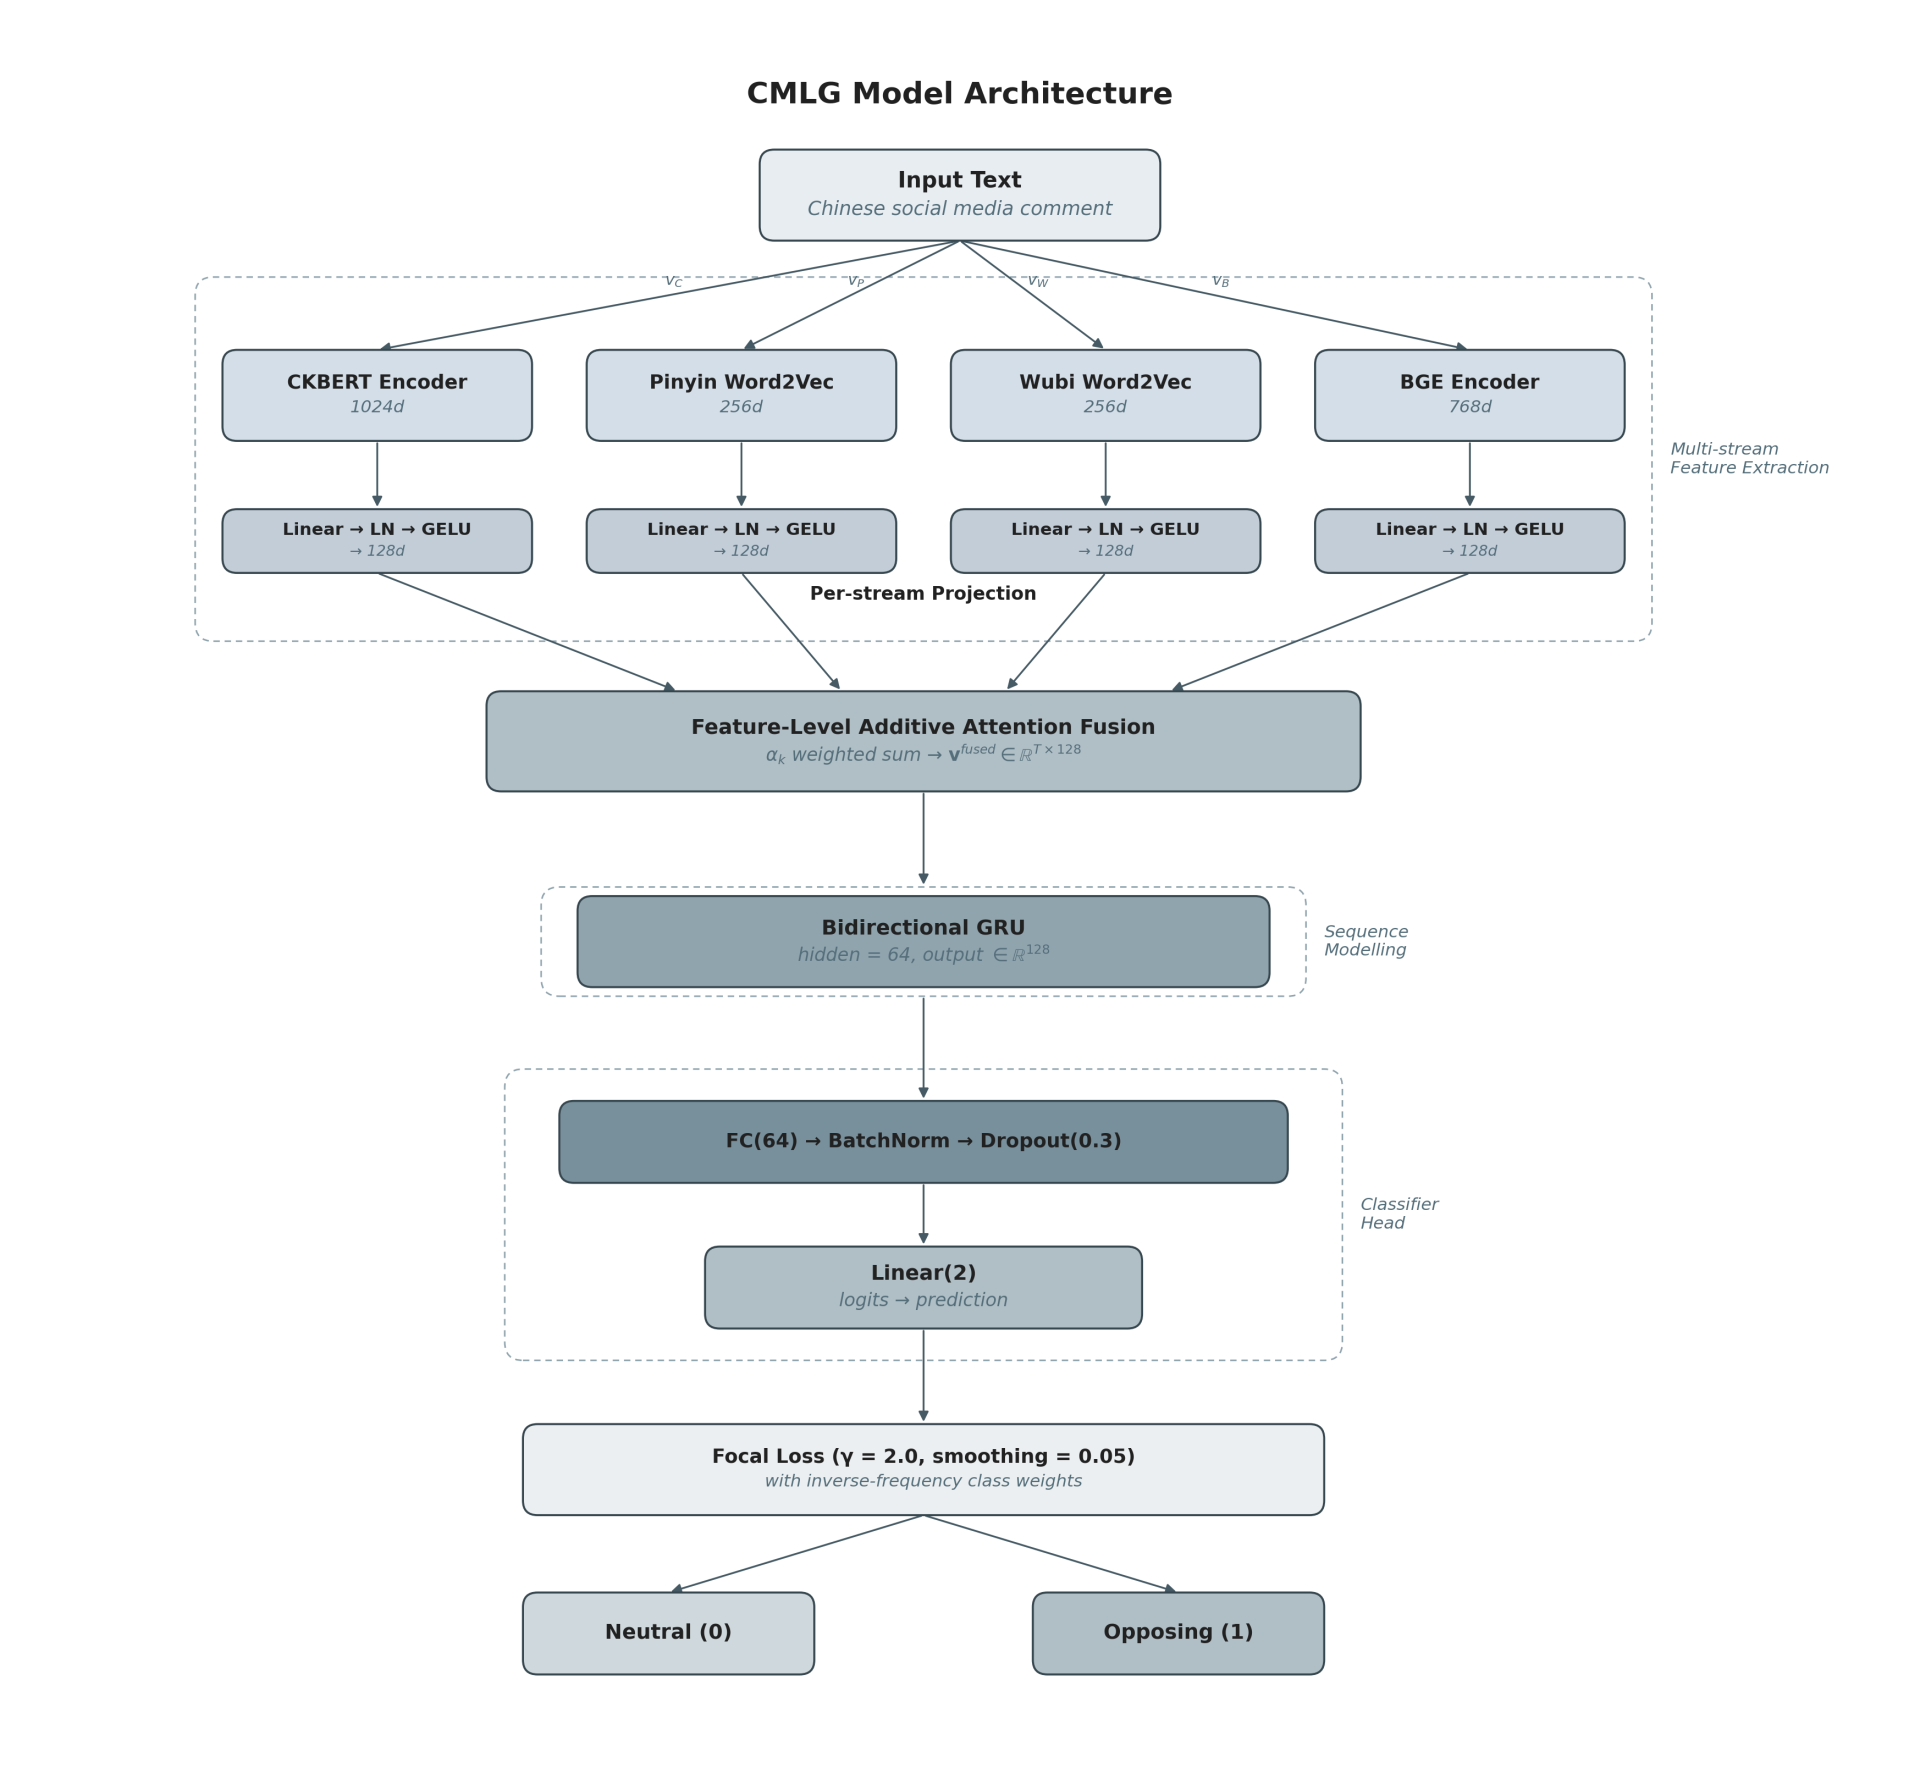
\includegraphics[width=0.78\textwidth]{model_architecture.png}
\caption{CMLG architecture. Four feature streams are projected to 128 dimensions, fused via additive attention, and classified by a Bi-GRU backbone.}
\label{fig:architecture}
\end{figure}

\subsection{Feature-Level Attention Fusion}
\label{sec:attention-fusion}
The four streams differ in dimensionality (1024, 768, 256, 256); naively concatenating them would let higher-dimensional streams dominate gradient updates. We address this with a two-stage fusion.

\textbf{Stage 1: Per-stream Projection.} Each stream $v_k$ ($k \in \{c, p, w, b\}$) is projected to a common dimensionality $d = 128$ via a learnable linear layer, Layer Normalization, and GELU activation:
\[
\hat{v}_k = \mathrm{GELU}\bigl(\mathrm{LayerNorm}(W_k \, v_k + b_k)\bigr), \quad \hat{v}_k \in \mathbb{R}^{T \times 128}
\]
where $W_k \in \mathbb{R}^{128 \times d_k}$ is the projection matrix for stream $k$ with original dimensionality $d_k$, and $b_k \in \mathbb{R}^{128}$ is the bias.

\textbf{Stage 2: Additive Attention.} Following Bahdanau et al.\ [15], we compute a scalar attention score for each stream at each character position $t$. The $K$ projected features ($K$ = number of active streams) are stacked into $\mathbf{H} \in \mathbb{R}^{T \times K \times 128}$, and attention weights are:
\[
\alpha_{t,k} = \frac{\exp\bigl(\mathbf{v}^\top \tanh(\mathbf{W}_a \, \hat{v}_{t,k})\bigr)}{\sum_{j=1}^{K} \exp\bigl(\mathbf{v}^\top \tanh(\mathbf{W}_a \, \hat{v}_{t,j})\bigr)}
\]
where $\mathbf{W}_a \in \mathbb{R}^{128 \times 128}$ is a learnable weight matrix and $\mathbf{v} \in \mathbb{R}^{128}$ is a learnable context vector. The fused representation is:
\[
v_t^{\mathrm{fused}} = \sum_{k=1}^{K} \alpha_{t,k} \, \hat{v}_{t,k} \in \mathbb{R}^{128}
\]
This lets the network emphasize whichever stream is most informative at each character position, rather than applying a fixed weighting.

\subsection{Classification Network}

The fused sequence $v^{\mathrm{fused}} \in \mathbb{R}^{T \times 128}$ passes through the following layers. A single-layer bidirectional GRU [21] with hidden size 64 per direction encodes the sequence; the final forward and backward hidden states are concatenated to produce $h_{\mathrm{GRU}} \in \mathbb{R}^{128}$. This vector enters a fully connected block: Linear($128 \to 64$) $\to$ BatchNorm(64) $\to$ ReLU $\to$ Dropout($p = 0.3$) $\to$ Linear($64 \to 2$). The output logits are used directly for prediction (argmax) and for loss computation. The total number of trainable parameters (excluding frozen CKBERT and BGE encoders) is approximately 150K, depending on the number of active streams.

\subsection{Training}
We optimize with AdamW [22] (lr $= 5 \times 10^{-4}$, weight decay $10^{-4}$, gradient clipping at norm 1.0). A ReduceLROnPlateau scheduler halves the learning rate if validation macro F1 does not improve for 7 epochs; training stops early after 20 epochs without improvement. Batch size is 64; maximum sequence length is 512 characters.

For class imbalance we use Focal Loss [11] with focusing parameter $\gamma = 2.0$ and label smoothing $\epsilon = 0.05$:
\[
\mathcal{L}_{\mathrm{focal}} = -\sum_{i} w_{y_i}\,(1 - p_{i,y_i})^{\gamma} \, \log\bigl((1-\epsilon)\,p_{i,y_i} + \epsilon/C\bigr)
\]
where $p_{i,y_i}$ is the predicted probability for the true class of sample $i$, $w_{y_i}$ is the inverse-frequency class weight, and $C=2$ is the number of classes. All results use stratified 5-fold cross-validation.

\section{Results}

\subsection{Experimental Setup}
All experiments use a single NVIDIA A100-SXM4-40GB GPU with PyTorch 2.5. Macro F1 under stratified 5-fold cross-validation is the primary metric; we also report accuracy, per-class F1, precision, and recall. We test five feature configurations---\textbf{only\_c} (CKBERT), \textbf{only\_b} (BGE), \textbf{c+b}, \textbf{c+p+w} (CKBERT + pinyin + wubi), and \textbf{c+p+w+b} (all four streams)---to isolate each stream's contribution. The same fold splits are reused across all configurations and dataset versions to ensure pairwise comparability.

\subsection{Ablation on the Original Dataset}

Table~\ref{tab:original-results} reports the 5-fold results on the original 8{,}969-sample corpus.

\begin{table}[htbp]
\centering
\caption{Ablation results on the original dataset (macro F1 $\pm$ std).}
\label{tab:original-results}
\begin{tabular}{lccccc}
\toprule
Setting & Accuracy & Macro F1 & F1 (Neutral) & F1 (Opposing) \\
\midrule
only\_c   & 0.8203 & 0.7796 $\pm$ 0.0108 & 0.8540 & 0.7136 \\
only\_b   & 0.8132 & 0.7709 $\pm$ 0.0101 & 0.8485 & 0.7020 \\
c+b       & 0.8248 & \textbf{0.7824 $\pm$ 0.0051} & 0.8554 & 0.7177 \\
c+p+w     & 0.8215 & 0.7803 $\pm$ 0.0075 & 0.8539 & 0.7148 \\
c+p+w+b   & 0.8208 & 0.7781 $\pm$ 0.0054 & 0.8531 & 0.7112 \\
\bottomrule
\end{tabular}
\end{table}

All five configurations fall within a narrow 1.2pp band (0.7709--0.7824), with c+b marginally ahead. The minority-class F1 hovers around 0.70--0.72, well below the neutral-class 0.85+, pointing to a bottleneck beyond class imbalance. Pinyin and wubi features provide no measurable benefit here: c+p+w trails c+b, and c+p+w+b ranks last among all configurations.

\subsection{Effect of Label Cleaning}

Table~\ref{tab:cleaned-results} reports the same five ablations on both cleaned variants.

\begin{table}[htbp]
\centering
\caption{Ablation results on the cleaned datasets (macro F1 $\pm$ std).}
\label{tab:cleaned-results}
\begin{tabular}{llcccc}
\toprule
Dataset & Setting & Accuracy & Macro F1 & F1 (Neutral) & F1 (Opposing) \\
\midrule
\multirow{5}{*}{\rotatebox{90}{Cleaned-Full}}
& only\_c   & 0.8264 & 0.8206 $\pm$ 0.0080 & 0.8527 & 0.7886 \\
& only\_b   & 0.8100 & 0.8023 $\pm$ 0.0127 & 0.8412 & 0.7635 \\
& c+b       & 0.8295 & 0.8209 $\pm$ 0.0066 & 0.8601 & 0.7817 \\
& c+p+w     & 0.8342 & \textbf{0.8259 $\pm$ 0.0104} & 0.8634 & 0.7885 \\
& c+p+w+b   & 0.8284 & 0.8198 $\pm$ 0.0072 & 0.8587 & 0.7808 \\
\midrule
\multirow{5}{*}{\rotatebox{90}{Cleaned-HC}}
& only\_c   & 0.9020 & 0.8958 $\pm$ 0.0064 & 0.9211 & 0.8704 \\
& only\_b   & 0.8824 & 0.8759 $\pm$ 0.0110 & 0.9043 & 0.8474 \\
& c+b       & 0.9042 & 0.8988 $\pm$ 0.0083 & 0.9221 & 0.8755 \\
& c+p+w     & 0.9068 & \textbf{0.9007 $\pm$ 0.0080} & 0.9253 & 0.8761 \\
& c+p+w+b   & 0.9024 & 0.8963 $\pm$ 0.0104 & 0.9215 & 0.8711 \\
\bottomrule
\end{tabular}
\end{table}

Moving from Original to Cleaned-Full, the best macro F1 rises from 0.7824 to 0.8259 (+4.4pp). Moving further to Cleaned-HC, it reaches 0.9007 (+12.0pp over Original). The minority-class F1 benefits even more: the best opposing-class F1 jumps from 0.7177 (Original) to 0.8761 (Cleaned-HC), a 15.8pp improvement. This asymmetry is consistent with minority-class samples being disproportionately affected by label noise, because annotators are more likely to disagree on the less prototypical class.

A noteworthy shift occurs in feature rankings. On the original data, c+b achieves the highest macro F1; on both cleaned variants, c+p+w takes the lead. This reversal indicates that the phonetic and structural features do carry discriminative information, but that information becomes learnable only when the training labels are sufficiently reliable.

\subsection{Cross-Dataset Comparison}

Table~\ref{tab:cross-dataset} juxtaposes macro F1 and minority-class F1 across datasets.

\begin{table}[htbp]
\centering
\caption{Cross-dataset comparison of macro F1 and opposing-class F1.}
\label{tab:cross-dataset}
\begin{tabular}{lccc|ccc}
\toprule
& \multicolumn{3}{c|}{Macro F1} & \multicolumn{3}{c}{F1 (Opposing)} \\
Setting & Original & Full & HighConf & Original & Full & HighConf \\
\midrule
only\_c   & 0.7796 & 0.8206 & 0.8958 & 0.7171 & 0.7886 & 0.8704 \\
only\_b   & 0.7709 & 0.8023 & 0.8759 & 0.7100 & 0.7635 & 0.8474 \\
c+b       & 0.7824 & 0.8209 & 0.8988 & 0.7267 & 0.7817 & 0.8755 \\
c+p+w     & 0.7803 & \textbf{0.8259} & \textbf{0.9007} & 0.7234 & \textbf{0.7885} & \textbf{0.8761} \\
c+p+w+b   & 0.7781 & 0.8198 & 0.8963 & 0.7181 & 0.7808 & 0.8711 \\
\midrule
Best      & c+b    & c+p+w  & c+p+w  & c+b    & c+p+w / c   & c+p+w \\
$\Delta$ vs Original & --- & +4.4pp & +12.0pp & --- & +6.2pp & +14.9pp \\
\bottomrule
\end{tabular}
\end{table}

The four-stream model (c+p+w+b) consistently underperforms c+p+w across all three datasets. Adding BGE on top of CKBERT, pinyin, and wubi hurts rather than helps, suggesting that the semantic overlap between CKBERT and BGE introduces redundancy that the additive attention mechanism cannot resolve. This observation aligns with the known limitation of additive attention: it computes an independent scalar weight per stream, without modeling pairwise interactions between streams.

Quality dominates quantity in these results. Cleaned-HC retains only 6{,}793 of the original 8{,}969 samples---a 24\% reduction---yet substantially outperforms both the full noisy set and the Cleaned-Full variant. Discarding ambiguous samples produces a cleaner decision boundary that more than compensates for the smaller training set.

\subsection{Baseline Comparison}

We compare CMLG against two baselines under identical evaluation conditions: (i)~SVM with character-level TF-IDF (trigram, 50K features, LinearSVC) and (ii)~BERT-base-chinese with full fine-tuning (5 epochs, lr $2\times10^{-5}$, max length 128). Table~\ref{tab:baselines} reports the results.

\begin{table}[htbp]
\centering
\caption{Comparison with baseline methods across three dataset versions.}
\label{tab:baselines}
\begin{tabular}{llcccc}
\toprule
Dataset & Method & Accuracy & Macro F1 & F1 (Neutral) & F1 (Opposing) \\
\midrule
\multirow{3}{*}{Original}
& SVM + TF-IDF          & 0.8009 & 0.7719 $\pm$ 0.0092 & 0.8532 & 0.6906 \\
& BERT-base-chinese (ft) & 0.8103 & 0.7935 $\pm$ 0.0090 & 0.8517 & 0.7353 \\
& CMLG (c+b)            & 0.8248 & 0.7824 $\pm$ 0.0051 & 0.8554 & 0.7177 \\
\midrule
\multirow{3}{*}{Cleaned-Full}
& SVM + TF-IDF          & 0.8120 & 0.7998 $\pm$ 0.0092 & 0.8492 & 0.7503 \\
& BERT-base-chinese (ft) & 0.8455 & \textbf{0.8399 $\pm$ 0.0100} & 0.8696 & 0.8102 \\
& CMLG (c+p+w)          & 0.8342 & 0.8259 $\pm$ 0.0104 & 0.8634 & 0.7885 \\
\midrule
\multirow{3}{*}{Cleaned-HC}
& SVM + TF-IDF          & 0.8762 & 0.8679 $\pm$ 0.0043 & 0.9010 & 0.8347 \\
& BERT-base-chinese (ft) & 0.9182 & \textbf{0.9128 $\pm$ 0.0039} & 0.9344 & 0.8911 \\
& CMLG (c+p+w)          & 0.9068 & 0.9007 $\pm$ 0.0080 & 0.9253 & 0.8761 \\
\bottomrule
\end{tabular}
\end{table}

BERT fine-tuning outperforms CMLG by 1.1--1.4pp in macro F1 across all datasets. This gap is consistent and statistically meaningful given the low standard deviations (0.004--0.010). The result is expected: BERT updates all 110M+ transformer parameters end-to-end, whereas CMLG freezes its pretrained encoders and trains only the projection, attention, and GRU layers (approximately 150K parameters). SVM trails both neural methods by a wider margin---5.5--9.6pp below BERT on the cleaned datasets---but still benefits substantially from label cleaning.

The cleaning effect is consistent across all three methods. SVM improves from 0.7719 to 0.8679 (+9.6pp), CMLG from 0.7824 to 0.9007 (+11.8pp), and BERT from 0.7935 to 0.9128 (+11.9pp) when moving from Original to Cleaned-HC. The near-identical magnitude of improvement across architecturally different models confirms that annotation quality, rather than model choice, is the primary constraint on this task. No amount of feature engineering or model scaling on the noisy data can match the gains from simply correcting the labels.

\section{Discussion}

\subsection{Orthographic Features and Label Quality}
The feature-ranking reversal between noisy and clean data is the central empirical finding of this work. On the original labels, pinyin and wubi features add nothing to classification performance; on cleaned labels, c+p+w consistently leads all configurations. This resolves an apparent contradiction with Ma et al.\ [9], who reported gains from character-form features on SWSR: the discrepancy likely reflects differences in noise levels between their processing pipeline and ours, or differences in how orthographic features are integrated into the model.

Mechanistically, the attention module learns to up-weight whichever stream is most informative at each character position. Under noisy supervision, gradient signals from mislabeled samples corrupt the attention weights, causing the fusion to degrade toward near-uniform averaging. When this happens, the subtle discriminative signal carried by pinyin and wubi embeddings is drowned out by the stronger but noisier gradients from the semantic streams. Once labels are corrected, the attention weights stabilize, and the model can exploit phonetic and structural cues---for instance, detecting that a character was substituted for a homophone of a gendered slur, or that a shape-similar glyph replaces a character in a derogatory term. These are precisely the evasion tactics that semantic embeddings alone cannot capture, because the embedding of the substitute character reflects its literal meaning rather than the intended offensive one.

\subsection{Why BERT Fine-tuning Outperforms CMLG}
BERT fine-tuning updates 110M+ parameters end-to-end, while CMLG trains only approximately 150K parameters on top of frozen encoders. The 1.1--1.4pp macro F1 gap in favor of BERT is modest given this three-orders-of-magnitude difference in trainable capacity. BERT's advantage likely comes from its ability to adapt internal representations to the task, while CMLG must rely on fixed pretrained features and compensate through its fusion and classification layers.

The trade-off is interpretability. CMLG's modular architecture makes it possible to isolate which feature streams contribute and how their utility depends on label quality---an analysis that monolithic fine-tuning does not support. The finding that orthographic features shift from useless to most valuable after cleaning would not have been discoverable from BERT fine-tuning experiments alone, because BERT lacks separate, inspectable feature channels. For researchers interested in understanding \emph{why} certain features matter for Chinese hate speech detection, rather than simply maximizing a leaderboard score, the multi-stream design offers analytical leverage that a single-encoder model cannot provide.

\subsection{Annotation Quality as the Dominant Factor}
The 12pp macro F1 gain from label cleaning---observed across all three methods (SVM, BERT, CMLG)---dwarfs anything achievable by changing features or models on the noisy data (total spread on Original: 1.2pp for CMLG configurations). This result aligns with the predictions of the label-noise literature [19,20]: when a non-trivial fraction of training labels are incorrect, improvements in annotation quality yield higher returns than architectural advances.

The quantity--quality trade-off reinforces this point. Cleaned-HC discards 24\% of the corpus through unanimous-agreement filtering, yet produces a far better training signal than retaining all samples. This is not simply a matter of removing hard examples; it reflects the removal of genuinely mislabeled data points that would otherwise push decision boundaries in the wrong direction. The practical implication is clear: for tasks where annotation guidelines are subjective---as is common in hate speech and sentiment analysis---investing effort in label verification is likely to deliver larger performance gains than investing in more sophisticated modeling.

\subsection{Limitations and Future Directions}
Several limitations should be acknowledged. The binary formulation collapses directional stance (pro-male vs.\ pro-female antagonism), limiting the downstream utility of the classifier for content moderation systems that need to distinguish attack targets. The three LLMs used for cleaning share similar pretraining paradigms (large-scale Chinese web text) and may make correlated errors on genuinely ambiguous samples, introducing systematic bias into the cleaned labels. We mitigated this risk by using models from three different organizations (Alibaba, Zhipu, DeepSeek), but the possibility of shared blind spots remains.

All data come from the SWSR corpus; cross-platform generalization to Douyin, Bilibili, or WeChat is untested. The consistent underperformance of c+p+w+b relative to c+p+w indicates that additive attention is insufficient for resolving high inter-stream redundancy, and more expressive fusion mechanisms---such as cross-attention between streams or gating networks---may be needed to benefit from all four streams simultaneously. Finally, our approach requires access to large LLM APIs for the cleaning step, which introduces cost and reproducibility concerns for researchers without such access.

\section{Conclusion}
This paper presented CMLG, a multi-stream classification model that fuses CKBERT contextual embeddings, BGE dense-semantic embeddings, pinyin phonetic vectors, and wubi structural vectors through learnable feature-level additive attention, followed by a Bi-GRU sequence encoder and a fully connected classifier. The model was designed to detect gender-antagonistic discourse in Chinese social media, with particular attention to the evasion tactics---homophonic substitution and shape-similar character swaps---that are characteristic of this domain.

To address the label noise present in the SWSR dataset, we developed a cleaning pipeline in which three heterogeneous large language models independently classify every sample, and predictions are aggregated by majority vote. This produced two cleaned dataset variants: Cleaned-Full (majority agreement, 8{,}962 samples) and Cleaned-HighConf (unanimous agreement, 6{,}793 samples). We evaluated CMLG, along with SVM and BERT baselines, across all three dataset versions using stratified 5-fold cross-validation.

The experiments yielded three principal findings. First, label cleaning raised macro F1 by 9--14 percentage points for every method tested, establishing annotation quality as the dominant factor in this classification task---more important than model architecture, feature selection, or training strategy. Second, Chinese orthographic features (pinyin and wubi) were ineffective under noisy labels but became the strongest feature configuration after cleaning, demonstrating that annotation quality directly gates the learnability of fine-grained linguistic cues. Third, retaining only unanimously agreed samples outperformed the full corpus despite a 24\% reduction in data volume, confirming that label quality matters more than dataset size when annotations are subjective.

Future work will pursue three directions: extending the framework to directional stance classification (distinguishing pro-male from pro-female antagonism), evaluating cross-platform generalization on data from Douyin and Bilibili, and exploring more expressive fusion mechanisms such as cross-attention or gating networks to better handle inter-stream redundancy.

% \appendix
% \section{LLM Cleaning Prompt}
% \label{app:prompt}
% The following Chinese prompt was sent identically to each of the three LLMs. Input texts exceeding 500 characters were truncated before querying.

% \begin{quote}
% \small
% 你是一个中文社交媒体文本分类专家，专门识别性别对立言论。

% 分类标准：

% - 性别对立言论（标签1）：针对特定性别群体的贬低、攻击、歧视、污名化、刻板印象强化、挑拨性别矛盾的言论。包括但不限于：使用性别歧视性称呼（如"婚驴""舔狗""小仙女"等讽刺性称呼）、将负面特征归因于某一性别、煽动性别对立情绪。

% - 中立言论（标签0）：不包含上述内容的普通评论，即使话题涉及性别议题，只要表达方式客观理性、不带攻击性，也属于中立。

% 注意：

% - 仅根据文本本身判断，不要推测发言者意图

% - 反讽、阴阳怪气的性别攻击也算对立言论

% - 讨论性别议题但不带攻击性的属于中立

% 请判断以下中文社交媒体评论是否为性别对立言论。

% 评论：\{text\}

% 请只回复一个数字：1（性别对立）或 0（中立）。
% \end{quote}

\section*{References}
\begin{enumerate}
\item X. Luo, B. Liang, Q. Wang, J. Li, E. Cambria, X. Zhang, Y. He, M. Yang, and R. Xu, ``A literature survey on multimodal and multilingual sexism detection,'' \textit{IEEE Trans. Comput. Social Syst.}, vol.~12, no.~5, pp.~3709--3727, 2025, doi: 10.1109/TCSS.2025.3561921.

\item B. Qin and X. Wang, ``The impact of gender antagonism online public opinion on contemporary college students and countermeasures,'' \textit{J. Langfang Norm. Univ. (Soc. Sci. Ed.)}, vol.~40, no.~2, pp.~95--102, 2024, doi: 10.16124/j.cnki.cn13-1390/c.2024.02.002.

\item L. Fontanella, B. Chulvi, E. Ignazzi, A. Sarra, and A. Tontodimamma, ``How do we study misogyny in the digital age? A systematic literature review using a computational linguistic approach,'' \textit{Humanit. Soc. Sci. Commun.}, vol.~11, no.~1, p.~478, Apr. 2024, doi: 10.1057/s41599-024-02978-7.

\item B. G. Gutam, S. C. D, J. N. Kumar, S. D. Babu, J. S. Babu, and M. S. Kumar, ``A machine learning and community-driven approach for feminist cyber resistance framework to mitigate online gender-based violence,'' in \textit{Proc. 4th OPJU Int. Technol. Conf. (OTCON)}, 2025, pp.~1--5, doi: 10.1109/OTCON65728.2025.11070859.

\item A. Singh, D. Sharma, and V. K. Singh, ``Misogynistic attitude detection in YouTube comments and replies: A high-quality dataset and algorithmic models,'' \textit{Comput. Speech Lang.}, vol.~89, Art. no. 101682, 2025, doi: 10.1016/j.csl.2024.101682.

\item M. N. Vivekananda, V. V. Malgi, and P. A. Shidlyali, ``Integrating transformers and hybrid machine learning models for automated sexism detection in online discourse,'' in \textit{Proc. Int. Conf. AMATHE}, 2025, pp.~1--6, doi: 10.1109/amathe65477.2025.11081244.

\item A. Mohasseb, E. Amer, F. Chiroma, and A. Tranchese, ``Leveraging advanced NLP techniques and data augmentation to enhance online misogyny detection,'' \textit{Appl. Sci.}, vol.~15, no.~2, Art. no. 856, Jan. 2025, doi: 10.3390/app15020856.

\item A. Jiang, X. Yang, Y. Liu, and A. Zubiaga, ``SWSR: A Chinese dataset and lexicon for online sexism detection,'' \textit{Online Social Netw. Media}, vol.~27, p.~100182, 2022, doi: 10.1016/j.osnem.2021.100182.

\item Z. Ma, S. Zhang, Y. Liu, and G. Zhang, ``A gender-opposition speech recognition method integrating multi-features and expression emotion dictionary,'' \textit{J. Data Acquis. Process.}, vol.~39, no.~3, 2024, doi: 10.16337/j.1004-9037.2024.03.017.

\item T. Zhang, J. Dong, J. Wang, C. Wang, A. Wang, Y. Liu, J. Huang, Y. Li, and X. He, ``Revisiting and advancing Chinese natural language understanding with accelerated heterogeneous knowledge pre-training,'' in \textit{Proc. EMNLP (Industry Track)}, 2022, pp.~1634--1645.

\item T.-Y. Lin, P. Goyal, R. Girshick, K. He, and P. Doll\'{a}r, ``Focal loss for dense object detection,'' in \textit{Proc. IEEE Int. Conf. Comput. Vis. (ICCV)}, 2017, pp.~2980--2988, doi: 10.1109/ICCV.2017.324.

\item J. Devlin, M.-W. Chang, K. Lee, and K. Toutanova, ``BERT: Pre-training of deep bidirectional transformers for language understanding,'' in \textit{Proc. NAACL-HLT}, 2019, pp.~4171--4186.

\item S. Xiao, Z. Liu, P. Zhang, and N. Muennighoff, ``C-Pack: Packaged resources to advance general Chinese embedding,'' in \textit{Proc. ACL}, 2024, pp.~2523--2535, doi: 10.18653/v1/2024.acl-long.138.

\item T. Mikolov, K. Chen, G. Corrado, and J. Dean, ``Efficient estimation of word representations in vector space,'' in \textit{Proc. ICLR Workshop}, 2013, arXiv: 1301.3781.

\item D. Bahdanau, K. Cho, and Y. Bengio, ``Neural machine translation by jointly learning to align and translate,'' in \textit{Proc. ICLR}, 2015, arXiv: 1409.0473.

\item P. Fortuna and S. Nunes, ``A survey on automatic detection of hate speech in text,'' \textit{ACM Comput. Surv.}, vol.~51, no.~4, Art. no. 85, Jul. 2018, doi: 10.1145/3232676.

\item T. Davidson, D. Warmsley, M. Macy, and I. Weber, ``Automated hate speech detection and the problem of offensive language,'' in \textit{Proc. ICWSM}, 2017, pp.~512--515.

\item C. Sun, X. Qiu, Y. Xu, and X. Huang, ``How to fine-tune BERT for text classification?'' in \textit{Chinese Computational Linguistics (CCL)}, Lecture Notes in Computer Science, vol.~11856, 2019, pp.~194--206, doi: 10.1007/978-3-030-32381-3\_16.

\item B. Fr\'{e}nay and M. Verleysen, ``Classification in the presence of label noise: A survey,'' \textit{IEEE Trans. Neural Netw. Learn. Syst.}, vol.~25, no.~5, pp.~845--869, 2014, doi: 10.1109/TNNLS.2013.2292894.

\item H. Song, M. Kim, D. Park, Y. Shin, and J.-G. Lee, ``Learning from noisy labels with deep neural networks: A survey,'' \textit{IEEE Trans. Neural Netw. Learn. Syst.}, vol.~34, no.~11, pp.~8135--8153, 2023, doi: 10.1109/TNNLS.2022.3152527.

\item K. Cho, B. van Merri\"{e}nboer, C. Gulcehre, D. Bahdanau, F. Bougares, H. Schwenk, and Y. Bengio, ``Learning phrase representations using RNN encoder--decoder for statistical machine translation,'' in \textit{Proc. EMNLP}, 2014, pp.~1724--1734, doi: 10.3115/v1/D14-1179.

\item I. Loshchilov and F. Hutter, ``Decoupled weight decay regularization,'' in \textit{Proc. ICLR}, 2019, arXiv: 1711.05101.

\end{enumerate}

\end{document}